%File: anonymous-submission-latex-2026.tex
\documentclass[letterpaper]{article} % DO NOT CHANGE THIS
\usepackage[submission]{aaai2026}  % DO NOT CHANGE THIS
\usepackage{times}  % DO NOT CHANGE THIS
\usepackage{helvet}  % DO NOT CHANGE THIS
\usepackage{courier}  % DO NOT CHANGE THIS
\usepackage[hyphens]{url}  % DO NOT CHANGE THIS
\usepackage{graphicx} % DO NOT CHANGE THIS
\urlstyle{rm} % DO NOT CHANGE THIS
\def\UrlFont{\rm}  % DO NOT CHANGE THIS
\usepackage{natbib}  % DO NOT CHANGE THIS AND DO NOT ADD ANY OPTIONS TO IT
\usepackage{caption} % DO NOT CHANGE THIS AND DO NOT ADD ANY OPTIONS TO IT
\frenchspacing  % DO NOT CHANGE THIS
\setlength{\pdfpagewidth}{8.5in} % DO NOT CHANGE THIS
\setlength{\pdfpageheight}{11in} % DO NOT CHANGE THIS
%
% These are recommended to typeset algorithms but not required. See the subsubsection on algorithms. Remove them if you don't have algorithms in your paper.
\usepackage{algorithm}
\usepackage{algorithmic}

% Mathematical packages
\usepackage{amsmath}
\usepackage{amssymb}
\usepackage{mathtools}
\usepackage{amsthm}
\usepackage{enumitem}
\usepackage{tikz}

% Define theorem-like environments
\newtheorem{definition}{Definition}[section]

%
% These are are recommended to typeset listings but not required. See the subsubsection on listing. Remove this block if you don't have listings in your paper.
\usepackage{newfloat}
\usepackage{listings}
\DeclareCaptionStyle{ruled}{labelfont=normalfont,labelsep=colon,strut=off} % DO NOT CHANGE THIS
\lstset{%
	basicstyle={\footnotesize\ttfamily},% footnotesize acceptable for monospace
	numbers=left,numberstyle=\footnotesize,xleftmargin=2em,% show line numbers, remove this entire line if you don't want the numbers.
	aboveskip=0pt,belowskip=0pt,%
	showstringspaces=false,tabsize=2,breaklines=true}
\floatstyle{ruled}
\newfloat{listing}{tb}{lst}{}
\floatname{listing}{Listing}
%
% Keep the \pdfinfo as shown here. There's no need
% for you to add the /Title and /Author tags.
\pdfinfo{
/TemplateVersion (2026.1)
}

\setcounter{secnumdepth}{0} %May be changed to 1 or 2 if section numbers are desired.

% The file aaai2026.sty is the style file for AAAI Press
% proceedings, working notes, and technical reports.
%

% Title

% Your title must be in mixed case, not sentence case.
% That means all verbs (including short verbs like be, is, using,and go),
% nouns, adverbs, adjectives should be capitalized, including both words in hyphenated terms, while
% articles, conjunctions, and prepositions are lower case unless they
% directly follow a colon or long dash
\title{Markovian Transformers for Informative Language Modeling}
\author{
    Anonymous Submission
}
\affiliations{
    % Anonymous submission - affiliations hidden
}

\begin{document}

\maketitle

\begin{abstract}
Chain-of-Thought (CoT) reasoning often fails to faithfully reflect a language model's underlying decision process. We address this by introducing a \emph{Markovian} language model framework that structurally enforces CoT text to be causally essential, factoring next-token prediction through an intermediate CoT and training it to predict future tokens independently of the original prompt. Within this framework, we apply an informativeness objective to ensure the CoT effectively supports predictions, achieving a 33.2\% absolute accuracy improvement on GSM8K with Llama 3.1 8B. Perturbation tests confirm stronger reliance on the CoT, while cross-model transfers indicate these reasoning traces generalize across interpreters. Our approach enhances both accuracy and interpretability, potentially extending CoT reasoning to arbitrarily long contexts and diverse tasks.
\end{abstract}

% Uncomment the following to link to your code, datasets, an extended version or similar.
% You must keep this block between (not within) the abstract and the main body of the paper.
% \begin{links}
%     \link{Code}{https://aaai.org/example/code}
%     \link{Datasets}{https://aaai.org/example/datasets}
%     \link{Extended version}{https://aaai.org/example/extended-version}
% \end{links}

\section{Introduction}
\label{sec:intro}
The rapid advancement of language models (LMs) has led to impressive performance on complex cognitive tasks~\citep{NEURIPS2020_1457c0d6}. Yet it is often unclear \emph{why} an LM arrives at a particular conclusion, causing issues in high-stakes applications. Traditional interpretability methods analyze hidden activations or attention patterns to extract ``explanations''. Modern LMs, however, already generate coherent text: we might hope \emph{prompting} the model to articulate its reasoning (``Chain-of-Thought'' or CoT)~\citep{wei2022chain} would yield a faithful record of its thought process. 

Unfortunately, CoT explanations can be \emph{unfaithful}. For example, \citet{turpin2023language} show that spurious in-context biases often remain hidden in the CoT, and \citet{lanham2023measuring} find that altering CoT text may not affect the final answer. Such observations indicate that standard CoTs are not ``load-bearing.''

In this work, we take a \emph{pragmatic} approach to interpretability, focusing on \emph{informativeness} over full faithfulness. Rather than insisting the CoT mirrors the model's entire internal process, we require that \emph{the CoT alone suffices to produce the final answer}. In other words, if we remove the original prompt and rely only on the CoT, the model should still reach the correct output. This makes the CoT \emph{causally essential} and \emph{fragile}: changing it necessarily alters the prediction.

What distinguishes our approach is the clear distinction between the model \emph{relying on its CoT} versus generating \emph{more informative CoTs}. While traditional approaches train models to generate better-quality CoTs, they don't fundamentally change how the model uses them. Our Markovian framework, by contrast, forces the model to process information through the CoT bottleneck, making the CoT not just informative but \emph{causally load-bearing} for prediction.

For instance, Mistral-7B's CoT on arithmetic tasks changed dramatically after training. \textbf{Before training}, it simply listed all numbers and their (incorrect) sum (e.g., ``Sum = 76 + 90 + 92 + ... = 2314''). \textbf{After training}, it performed correct step-by-step calculations (e.g., ``calculate 6 + 89 = 95; Next, calculate 95 + 38 = 133...''), breaking the task into manageable steps that can be verified independently and enabling accurate answer prediction even when the original question is removed.

A key insight is that an \emph{informative} CoT can also serve as a \emph{recipient-specific compression} of the model's hidden knowledge: it distills the essential reasoning into text that another recipient (e.g.\ a different model or a human) can use to predict the same outcome. Our experiments confirm that the learned CoTs generalize across interpreters, suggesting that these textual explanations genuinely encode transferable problem-solving steps rather than model-specific quirks.

\subsection{Contributions}
\begin{enumerate}
    \item We introduce a Markovian language model framework that structurally enforces Chain-of-Thought (CoT) generation to be causally essential, ensuring reliance on the CoT for predictions.
    \item We apply this framework to arithmetic problems (Mistral 7B) and the GSM8K dataset~\citep{cobbe2021gsm8k} (Llama 3.1 8B), observing a 33.2\% absolute improvement on GSM8K.
    \item We show that perturbing the CoT consistently degrades prediction accuracy, verifying \emph{fragility} and causal relevance.
    \item We demonstrate cross-model transfer: CoTs trained on one model remain informative for other models. This underscores the CoT's \emph{recipient-specific} interpretability and suggests it captures a shared reasoning strategy.
\end{enumerate}

\begin{figure*}[t!]
  \centering
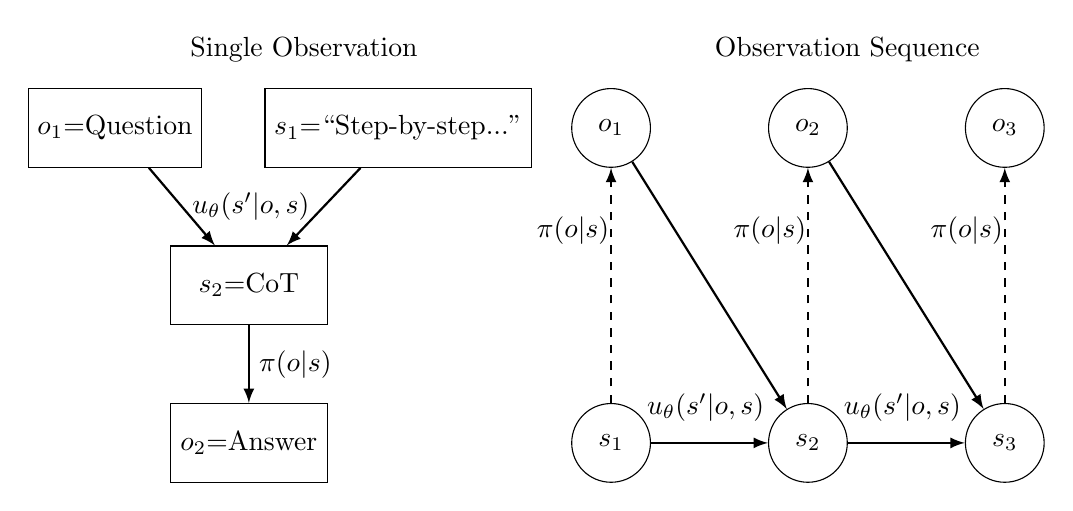
\begin{tikzpicture}[
    node distance=2cm,
    box/.style={rectangle, draw, minimum width=2cm, minimum height=1cm},
    circlebox/.style={circle, draw, minimum size=1cm},
    arrow/.style={->, thick},
    >=latex
]

% Left side: Single timestep
\node[box] (Q) at (-4.3,2) {$o_1$=Question};
\node[box] (S) at (-0.7,2) {$s_1$=``Step-by-step...''};
\node[box] (CoT) at (-2.6,0) {$s_2$=CoT};
\node[box] (A) at (-2.6,-2) {$o_2$=Answer};

\draw[arrow] (Q) -- node[right] {$u_\theta(s'|o,s)$} (CoT);
\draw[arrow] (S) -- (CoT);
\draw[arrow] (CoT) -- node[right] {$\pi(o|s)$} (A);

% Right side: Causal structure
% Observations
\node[circlebox] (o1) at (2,2) {$o_1$};
\node[circlebox] (o2) at (4.5,2) {$o_2$};
\node[circlebox] (o3) at (7,2) {$o_3$};

% States
\node[circlebox] (s1) at (2,-2) {$s_1$};
\node[circlebox] (s2) at (4.5,-2) {$s_2$};
\node[circlebox] (s3) at (7,-2) {$s_3$};

% Connections
\draw[arrow] (o1) to (s2);
\draw[arrow] (s1) to (s2);
\node[above] at (3.2,-1.85) {$u_\theta(s'|o,s)$};

\draw[arrow] (o2) to (s3);
\draw[arrow] (s2) to (s3);
\node[above] at (5.7,-1.85) {$u_\theta(s'|o,s)$};

% π(o|s) connections
\draw[arrow, dashed] (s1) to (o1);
\node[left] at (2.1,0.7) {$\pi(o|s)$};

\draw[arrow, dashed] (s2) to (o2);
\node[left] at (4.6,0.7) {$\pi(o|s)$};

\draw[arrow, dashed] (s3) to (o3);
\node[left] at (7.1,0.7) {$\pi(o|s)$};

% Labels
\node at (-1.9,3) {Single Observation};
\node at (5,3) {Observation Sequence};

\end{tikzpicture}
\caption{Illustration of the Markovian framework. Left: Single time-step process from Question to CoT to Answer. Right: Causal structure showing the generation of states from observations and previous states using $u_\theta(s'|o,s)$, and prediction of observations from states using $\pi(o|s)$. In experiments, both $u_\theta$ and $\pi$ use the same transformer, but only $u_\theta$ weights are updated during training.}
\label{fig:markovian-framework}
\end{figure*}

\section{Related Work}
\label{sec:related_work}

Prior work shows that CoT prompting can boost performance on reasoning tasks~\citep{wei2022chain}. Whereas typical CoT prompting methods do not alter a pre-trained model's parameters, some prior approaches do fine-tune the model for CoT generation. Our work differs by removing the original question or passage from the answer-prediction context, which enforces a stronger causal reliance on the CoT.

Regarding faithfulness vs. interpretability, some authors discuss how a CoT may fail to reflect the true reason the LM arrived at its answer~\citep{lanham2023measuring, turpin2023language}, since small changes in the CoT do not necessarily change the final prediction. We build on these insights by \emph{training} the model to rely on this channel exclusively.

Architecturally, our Markovian LM shares structural similarities with state space models like RNNs~\citep{rumelhart1986learning}, though with a key difference: MLMs have probabilistic state transitions to model token sampling, which necessitates gradient estimation methods such as policy gradient rather than direct backpropagation. This probabilistic structure also resembles Kalman filters and Variational Recurrent Neural Networks (VRNN), though we use categorical rather than Gaussian distributions for interpretable text generation. Other fine-tuned reasoning models have similar structure but allow seeing the full context before generating state/reasoning tokens, whereas our approach enforces a strict information bottleneck through the state.

\citet{lyu2023faithful} also consider restricting the model's ability to see the original input while generating the final answer. Their approach, however, involves rewriting the question in a structured formal language or code that is then executed. Our approach uses natural language for the reasoning state to preserve interpretability across diverse tasks.

\section{Markovian Language Models and Informativeness}
\label{sec:MLM}

Here we provide our formalism for Markovian Language Models (MLMs) and define \emph{informativeness}, which we use as a training objective within our novel structural framework.

\subsection{Markovian Language Models (MLM)}

A traditional LM can attend to the entire context when predicting the next token. This makes it possible for an LM to disregard the CoT or only partially rely on it. We impose a stricter, \emph{Markovian} structure:

\begin{definition}[Markovian LM]
A Markovian Language Model is a tuple $M=(\mathcal{O}, \mathcal{S}, \pi, u, s_1)$, where
\begin{itemize}
\item $\mathcal{O}$ is a set of observations (e.g., questions and answers in a QA task),
\item $\mathcal{S}$ is a set of states (e.g., CoT reasoning text),
\item $\pi: \mathcal{S}\rightarrow \Delta(\mathcal{O})$ is a policy that predicts the next observation from the state alone,
\item $u: \mathcal{O}\times\mathcal{S}\rightarrow \Delta(\mathcal{S})$ is a state update function (produces CoT from question and initial prompt),
\item $s_1\in \mathcal{S}$ is an initial state (starting CoT prompt).
\end{itemize}
\end{definition}

For example, in a math reasoning task, $o_1 \in \mathcal{O}$ might be a question, $s_1 \in \mathcal{S}$ is an initial CoT prompt like ``Let's solve this step-by-step:'', $s_2 \in \mathcal{S}$ is the generated reasoning chain, and $o_2 \in \mathcal{O}$ is the answer. The key idea is that $\pi$ can only see the CoT state $s_2$ when predicting $o_2$, forcing the CoT to contain all needed information. Intuitively, $\pi$ is the \emph{frozen} next-token predictor, and $u$ is the model's \emph{trainable} component that chooses how to produce the CoT from the latest observation and prior state. In our experiments, $\pi$ and $u$ share the same underlying transformer but we freeze the weights for $\pi$ while fine-tuning those used by $u$. 

\subsection{Data-Generating Distribution and Reward}

Let $P$ be the distribution over observations $x_1, x_2, \dots, x_T \in \mathcal{O}$. A trajectory $\tau$ is generated by:
\[
s_{t+1}\sim u(s_t, x_t), \quad x_{t+1}\sim P(x_{t+1}\mid x_{\le t}),
\]
with $s_1$ a fixed initial prompt. We define the \emph{reward} for a trajectory $\tau$ as:
\[
R(\tau)=\sum_{t=1}^T \left[\ln \pi(x_t\mid s_t)-\ln \pi(x_t\mid s'_t)\right],
\]
where $s'_t$ is generated by a \emph{baseline} update function $u'$, e.g., the \emph{untrained} model. In words, $R(\tau)$ measures how much more likely the correct observation $x_t$ is under the trained state $s_t$ compared to the baseline state $s'_t$.

\subsection{Informativeness Objective}

Conceptually, we aim to ensure that the CoT state serves as a critical bottleneck for information flow, making it causally essential for predictions. Formalizing this within our Markovian framework, we define:
\[
  J(\theta)=\mathbb{E}_{\tau \sim P,u_\theta,u'}\left[R(\tau)\right],
\]
where $\theta$ parameterizes $u_\theta$. Maximizing $J(\theta)$ ensures that the update function $u_\theta$ produces states $s_t$ that are \emph{informative} about future observations (relative to the baseline $u'$), thereby enforcing the CoT's role as a load-bearing component. We optimize $J(\theta)$ with policy gradient or PPO, sampling observations from $P$ and states from $u_\theta$ and $u'$.

\section{Methods}
\label{sec:method}
\subsection{Implementation as Question-Answer Pairs}
In many tasks like math problem solving, we have $T=2$ observations (question and answer) and implement the abstract MLM with a fixed maximum length for the CoT state. Let $\mathcal{V}$ be a token vocabulary. We set $\mathcal{O} = \mathcal{V}^N$ and $\mathcal{S} = \mathcal{V}^K$ for some $N, K \in \mathbb{N}$, where $K$ is the maximum tokens in the CoT. Note that while we limit the state to a maximum of $K$ tokens for implementation, we do not enforce fixed-length observations. 

Our conceptual arguments rely on $K < N$, as otherwise the model could simply write the predicted observation into the state. We satisfy this in our Wikipedia experiments, and for other experiments we find empirically that the model does not learn this undesirable behavior due to the difficulty of predicting the answer directly without any CoT.

In this setting, we denote our states as $s_1 = \text{CoT}_{\text{init}}$ and $s_2 = \text{CoT}$, where $\text{CoT}_{\text{init}}$ is a task-specific prompt. With pre-trained LM $\mathcal{L}$, we implement our update function $u$ as:
\begin{align}
\ln u\bigl(s_2 = \text{CoT} \,\mid\, q, s_1 = \text{CoT}_{\text{init}}\bigr) &= 
\sum_{i=1}^{K} \ln \mathcal{L}(c_i)\bigl[\text{CoT}_i\bigr]
\end{align}
where $c_i = \text{concat}(q, \text{CoT}_{\text{init}}, \text{CoT}_{<i})$. The policy $\pi$ is implemented as:
\begin{align}
\ln \pi(\text{ans} \mid \text{CoT}) &=  \sum_{i=1}^{N} \ln \mathcal{L}(d_i) [\text{ans}_i]
\end{align}
where $d_i = \text{concat}(\text{CoT}, \text{ans}_{<i})$.

Crucially, we do \emph{not} allow the answer generation to attend back to the question $q$ directly; the question is replaced by the $\text{CoT}$. For each question $q$, we generate the baseline state $s'_2$ (which we denote as $\text{CoT}'$ in this setting) by prompting the unmodified pre-trained model with $q$ plus an initial instruction (e.g., 'Think step-by-step...'), and recording its raw output.

Our reward is:
\[
R = \ln \pi(\text{ans} \mid \text{CoT}) \;-\; \ln \pi(\text{ans} \mid \text{CoT}').
\]

\subsection{Reinforcement Learning Objectives}
\label{subsec:rl_objectives}
Having defined the reward in terms of CoT informativeness, we explore three RL techniques to optimize $u_\theta$ toward producing high-reward CoTs. All three rely on sampling $\text{CoT}$ and $\text{CoT'}$ for a given question $q$, then comparing their contributions to the final answer likelihood. 

\subsubsection{Threshold-based Expert Iteration (TEI)}
\label{subsubsec:tei}
Threshold-based Expert Iteration consists of the following steps:
\begin{enumerate}
    \item Sample $\text{CoT}$ from the trained policy $u_\theta$ and a baseline $\text{CoT'}$ from $u'$ for the same question $q$.
    \item Estimate informativeness $I(\text{ans}, \text{CoT}, \text{CoT'}) \;=\; \pi(\text{ans}\mid \text{CoT}) \;-\; \pi(\text{ans}\mid \text{CoT'})$.
    \item If $I$ is at least one standard deviation above the historical average:
\begin{itemize}
            \item Compute $\nabla_\theta \ln u_\theta(\text{CoT} \mid q, \text{CoT}_{\text{init}})$.
            \item Perform gradient ascent on $\theta$.
\end{itemize}
\end{enumerate}
\noindent
\textbf{Limitation:} TEI discards CoTs that yield moderate but still valuable rewards, potentially slowing learning.

\subsubsection{Policy Gradient (PG)}
\label{subsubsec:pg}
Policy Gradient with thresholding extends TEI by weighing updates by $I$:
\begin{enumerate}
    \item Sample $\text{CoT}$ and a baseline $\text{CoT'}$ for each question $q$.
    \item Compute $I = \pi(\text{ans}\mid \text{CoT}) - \pi(\text{ans}\mid \text{CoT'})$.
    \item If $I$ is at least one standard deviation above its historical mean:
\begin{itemize}
            \item Calculate $\nabla_\theta \ln u_\theta(\text{CoT} \mid q, \text{CoT}_{\text{init}})$.
            \item Scale this gradient by $I$ and ascend.
\end{itemize}
\end{enumerate}
\noindent
\textbf{Advantage:} Uses more of the reward signal, accelerating learning. \\
\textbf{Disadvantage:} Potentially more instability, especially if $I$ is large or negative.

\subsubsection{Proximal Policy Optimization (PPO)}
\label{subsubsec:ppo}
PPO clips probability ratios to stabilize large policy updates:
\begin{enumerate}
    \item For a sampled CoT $\text{CoT}$, compute the ratio $r = \frac{u_\theta(\text{CoT}\mid q,\text{CoT}_{\text{init}})}{u'(\text{CoT}\mid q,\text{CoT}_{\text{init}})}$.
    \item Let $I = \pi(\text{ans}\mid \text{CoT}) - \pi(\text{ans}\mid \text{CoT'})$ be the informativeness reward.
    \item Define the clipped objective:
    \[
    \text{obj} = \min\!\Bigl(r \cdot I, \;\text{clip}(r,1-\epsilon,1+\epsilon)\cdot I\Bigr), 
     \text{where } \epsilon=0.2.
    \]
    \item Ascend on $\nabla_\theta \text{obj}$.
\end{enumerate}
\textbf{Key Idea:} PPO discourages the new CoT distribution $u_\theta$ from diverging too sharply from $u'$, thus trading off exploration and stability.


\section{Experiments}
\label{sec:experiments}

\begin{figure*}
\centering
    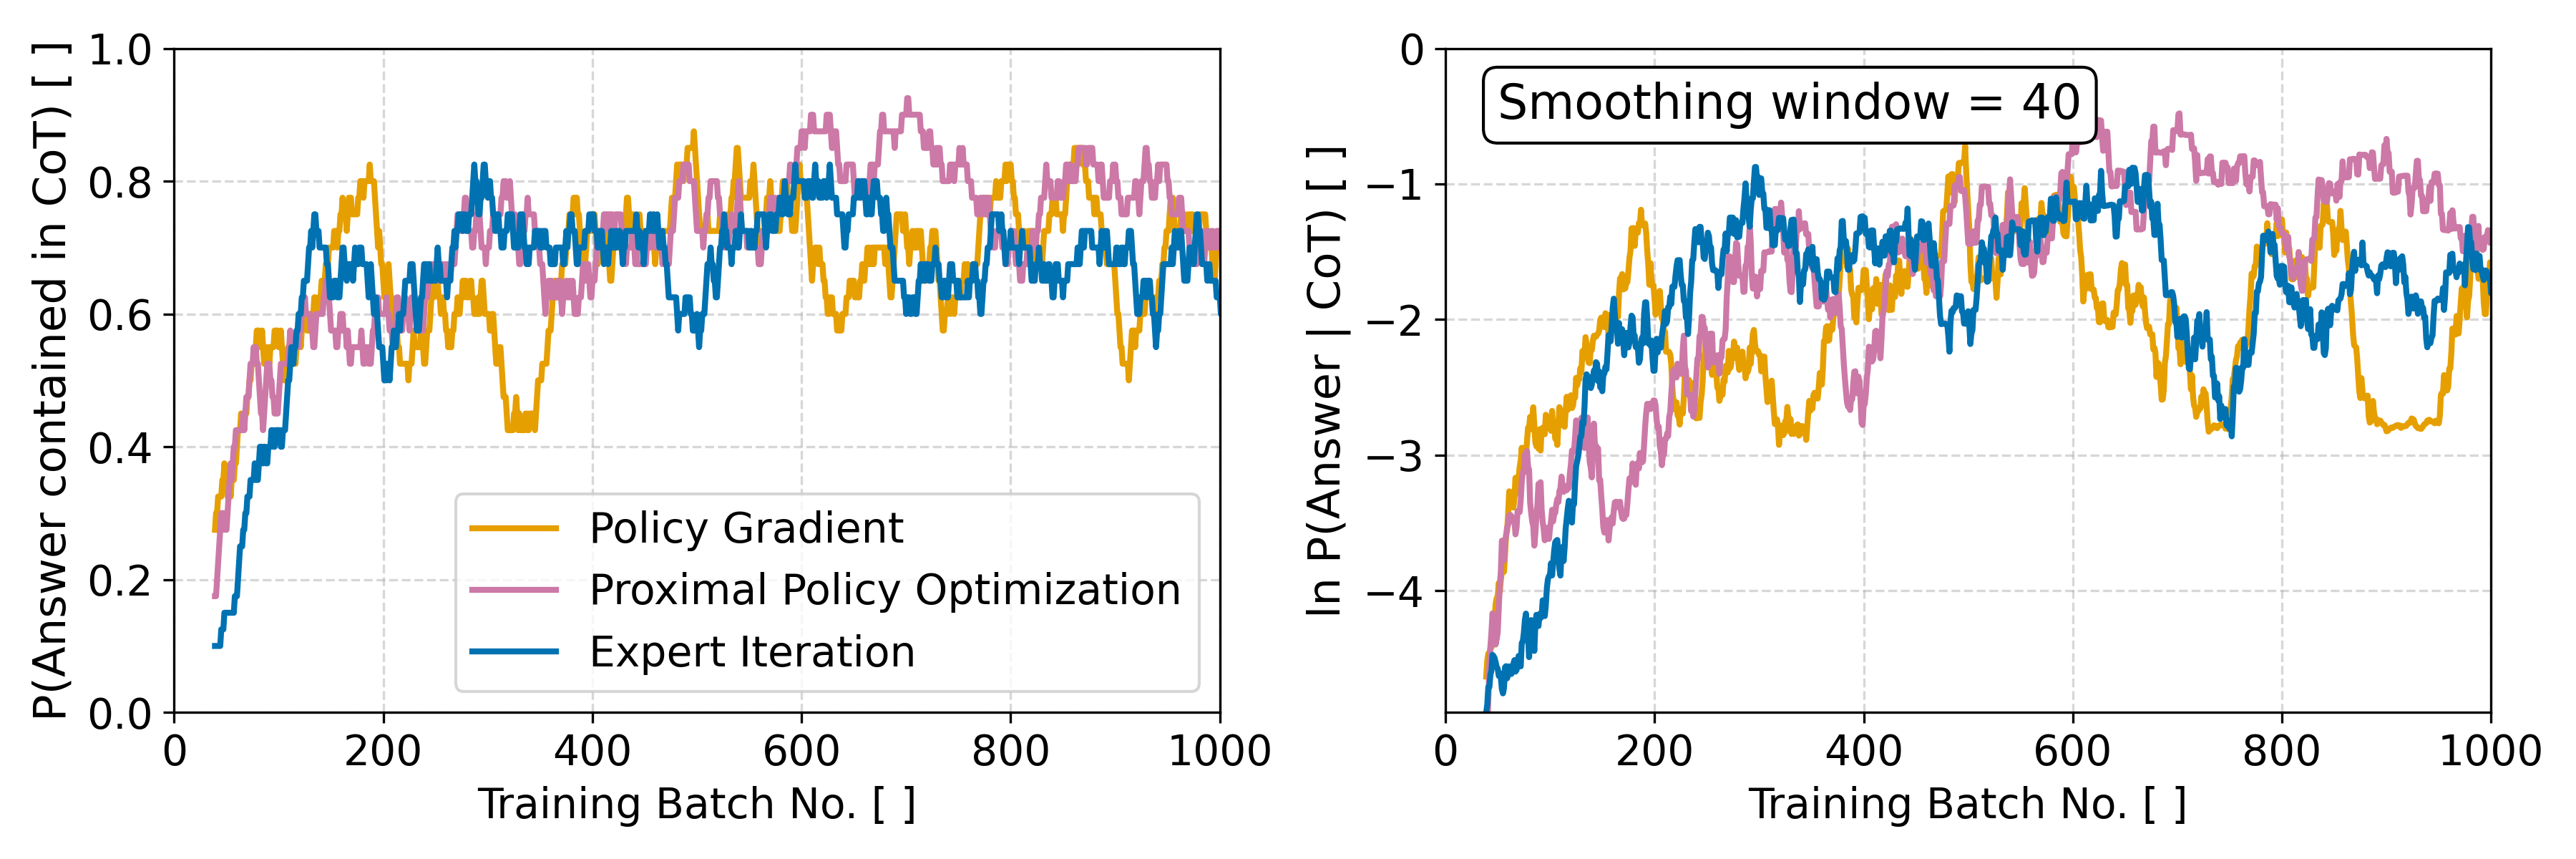
\includegraphics[width=\textwidth]{Figures/cot_performance_comparison.png}
    \caption{Training performance on multi-step addition. The log probability $\ln \pi(\text{ans} \mid \text{CoT})$ of the answer given a CoT, where CoT is sampled from trained weights and $\text{CoT}'$ from unmodified weights. We train to produce CoTs sufficient to predict the correct answer without the original question. This plot shows training of Mistral 7B Instruct V0.2 on fifteen-term addition problems. Due to high variance, we plot the point-wise maximum over four runs for each training technique.}
    \label{fig:arithmetic-results}
\end{figure*}

\subsection{Multi-step Addition}
\label{subsec:solving}
We generate random addition problems, where each problem consists of fifteen terms and each term is a uniform random natural number less than 100. We fine-tune Mistral 7B Instruct V0.2 to produce CoT tokens such that a frozen copy of the pre-trained language model can predict the correct answer given that CoT, for each training technique. As shown in Figure~\ref{fig:arithmetic-results}, PPO, our preferred training method for arithmetic, can mention the correct answer in up to 90\% of CoTs and achieve an average natural log probability of around -0.7. 

Since the Mistral tokenizer allocates a separate token for each digit, a natural log probability of -0.7 corresponds to about 50\% probability per token. The seeming contradiction between 90\% verbatim answer likelihood and 50\% per-digit uncertainty stems from the predictor's format uncertainty—it distributes probability across the entire vocabulary when deciding what follows "Answer:", as we only train CoT production $u_\theta(s'|o,s)$, not the predictor $\pi(o|s)$.

\begin{figure*}[ht]
\centering
    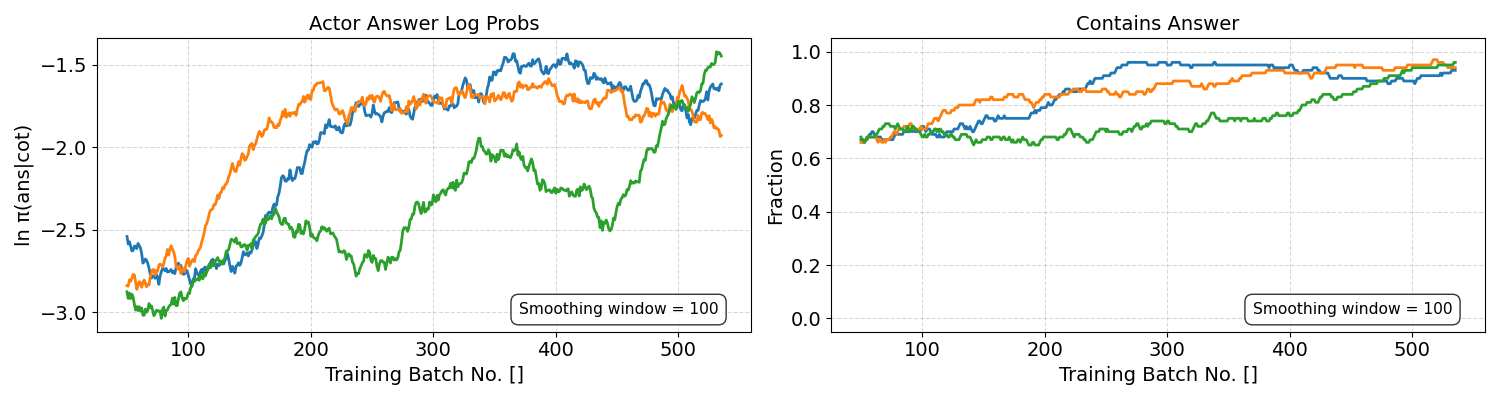
\includegraphics[width=\textwidth]{Figures/llama_combined_metrics_gsm8k.png}
    \caption{GSM8K performance metrics over three separate training runs of Llama-3.1-8B-Instruct. The left plot shows the log probability that an untrained Llama assigns to the correct answer given the trained CoT ($\ln \pi(\text{ans}|\text{CoT})$), and the right plot shows the proportion of CoTs in a batch which contain the answer verbatim. We use a smoothing window of size 100.}
    \label{fig:gsm8k-performance}
\end{figure*}

\subsection{GSM8K}
\label{subsec:gsm8k}
To test our method on more complex reasoning tasks, we train Llama-3.1-8B-Instruct on GSM8K using policy gradient with expert iteration (threshold 2.2 standard deviations) and a KL penalty (0.1). We produce up to 150 CoT tokens and estimate the value function with an exponentially decaying average of previous rewards (decay 0.9).

As shown in Figure~\ref{fig:gsm8k-performance}, we observe a dramatic increase in exact-match accuracy from 35.94\% baseline to 69.14\% in our best run—a 33.2\% absolute improvement. The other runs (58.23\% and 62.85\%) confirm consistent effectiveness on mathematical reasoning.

\subsection{Wikipedia}
\label{subsec:wikipedia}

We also explored applying our approach to general language modeling using Wikipedia text. For each article, we condition on the first 200 tokens and task the model with predicting the following 100 tokens, allowing 50 tokens of CoT to aid prediction. Training parameters match those used in GSM8K.

Results showed modest improvements in next-token prediction accuracy from 8.2\% to 10.5\%. This should be contextualized against pre-trained Llama's typical 16.9\% accuracy (over 10,000 articles) on the 200th to 300th tokens without context. The lower baseline (8.2\%) likely stems from our setup with CoT followed by " Answer: " before prediction. Despite this, key findings about CoT reliability remain evident: perturbing trained CoTs degrades accuracy more than perturbing baseline CoTs, indicating genuine CoT reliance.

\begin{figure*}[ht]
  \centering
  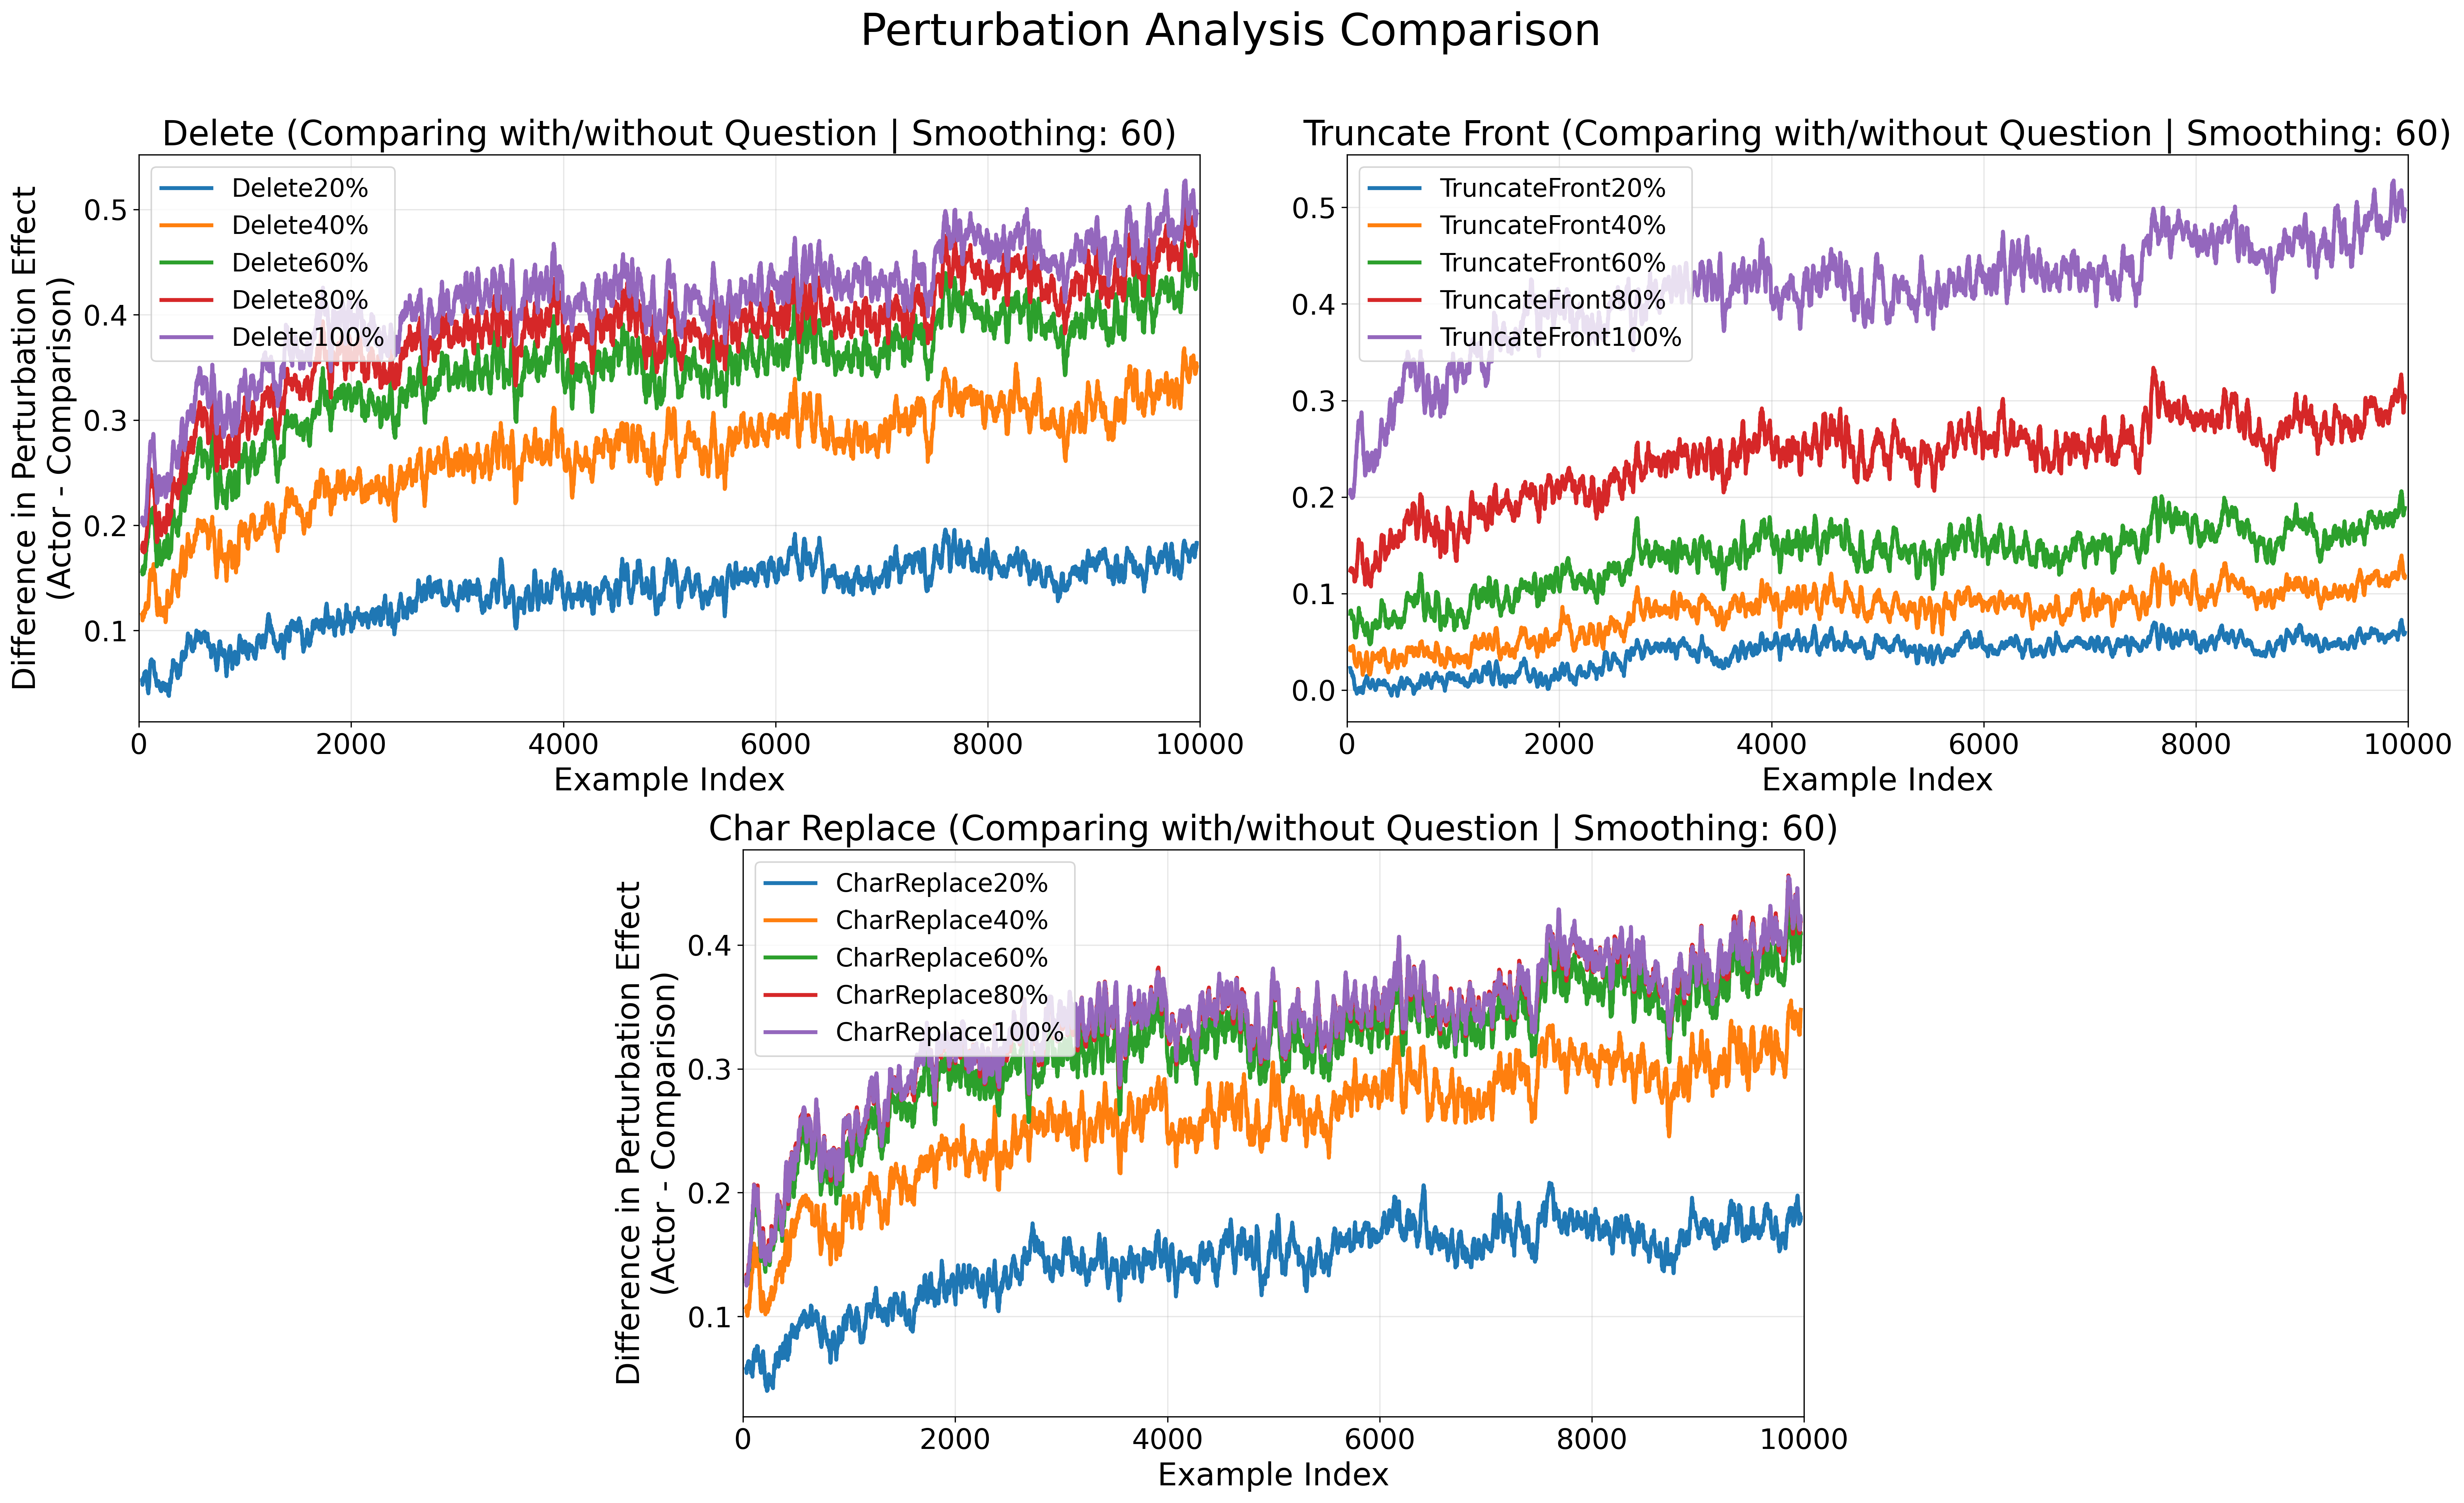
\includegraphics[width=\textwidth]{Figures/combined_perturbation_plot_comparison_question_centered.png}
  \caption{Impact of perturbations on CoT effectiveness with/without the original question. Three perturbation types shown: character deletion, front truncation, and random replacement. Higher values indicate stronger reliance on CoT when the question is absent, showing causal dependence rather than just improved accuracy.}
  \label{fig:perturbation}
\end{figure*}

\subsection{Measuring Fragility of CoT}\label{subsec:fragile}

Expanding upon \citet{lanham2023measuring}, we gauge model dependence on CoT tokens using three perturbations: character deletion, front truncation, and random character replacement.
    
To isolate genuine fragility from improved accuracy, we use a question-centered metric that compares perturbation effects with and without the original question:
\begin{align}
m_2 &= [\ln P(\text{ans}|\text{CoT}) - \ln P(\text{ans}|\text{perturb}(\text{CoT}))] \nonumber\\
&- [\ln P(\text{ans}|q, \text{CoT}) - \ln P(\text{ans}|q, \text{perturb}(\text{CoT}))]
\end{align}

As shown in Figure~\ref{fig:perturbation}, this metric directly measures how much the model relies on the CoT when the question is absent versus present. This difference increases significantly during training, confirming that our CoTs become genuinely more load-bearing rather than simply more accurate.

\begin{figure*}[ht]
  \centering
  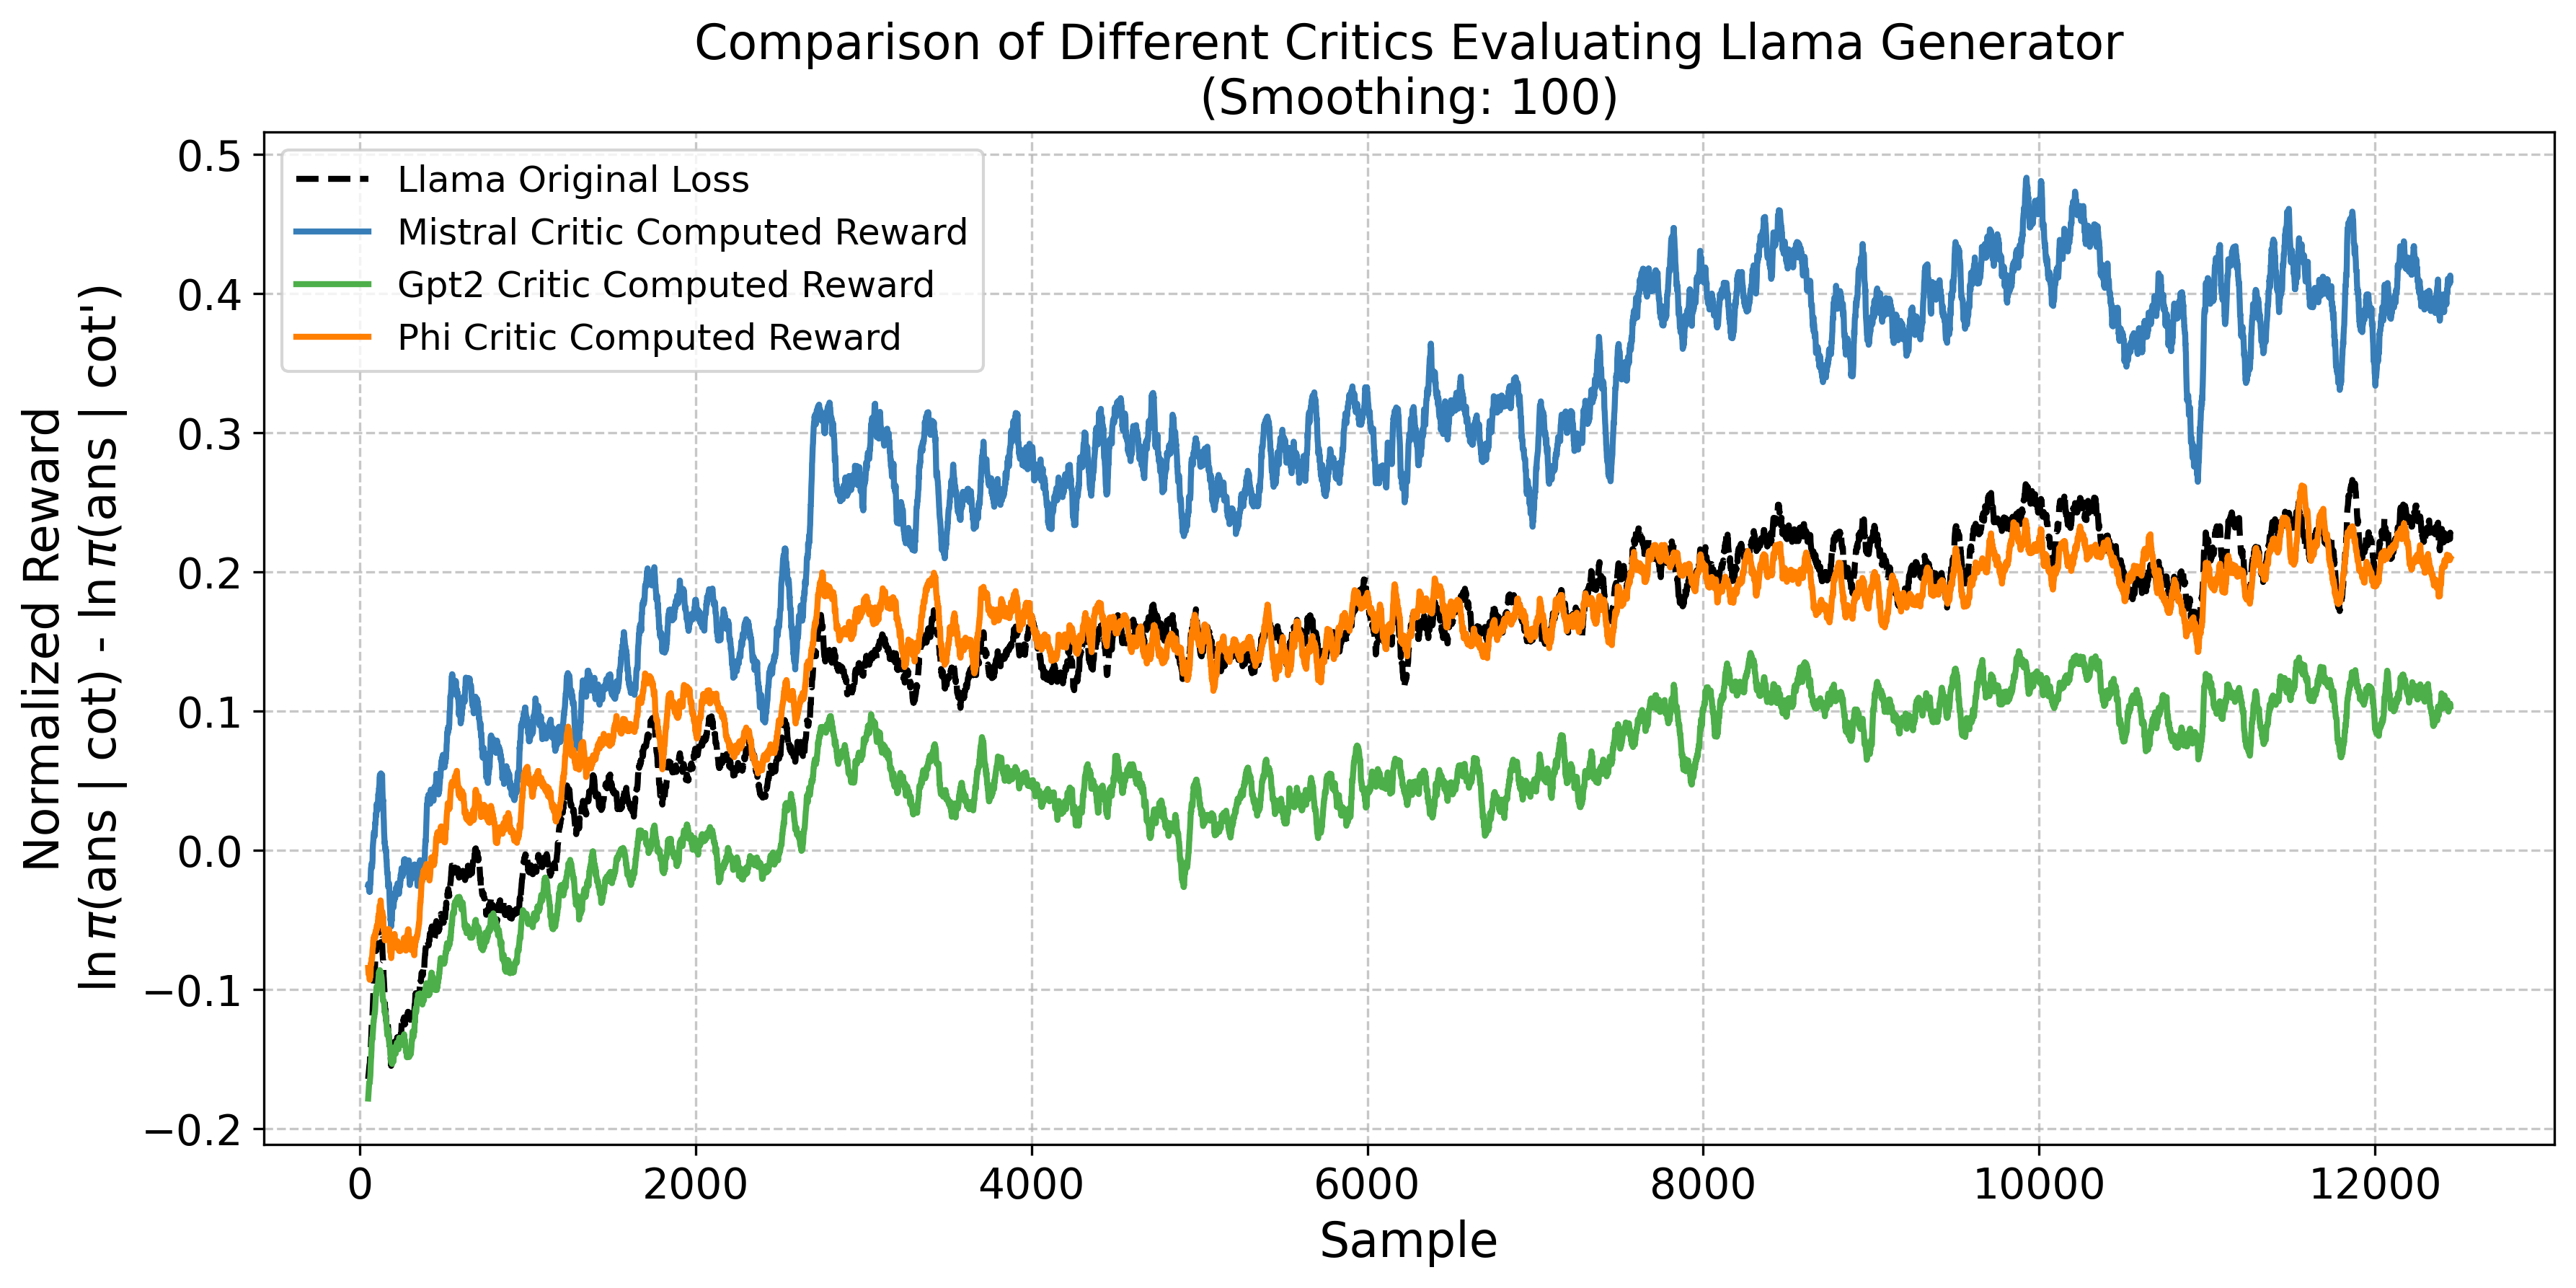
\includegraphics[width=.9\textwidth]{Figures/wiki_multi_critic_comparison.png}
  \caption{Cross-model evaluation showing Llama-3.1-8B-Instruct's evaluation of Mistral's CoT quality throughout training on Wikipedia text prediction. The correlation between improvements in both models' evaluations suggests the learned reasoning patterns generalize across architectures rather than being model-specific artifacts. Each plot is averaged across 6 independent training runs.}
  \label{fig:cross-eval}
\end{figure*}

\subsection{Interpretability of CoT Generations}
\label{subsec:interp}

To probe how well the reasoning generalizes, we evaluate CoT informativeness across different language models on the Wikipedia dataset. As shown in Figure~\ref{fig:cross-eval}, we test across three distinct model families (Phi, Mistral, and GPT2), including GPT2, a significantly smaller model that shouldn't be able to decode sophisticated steganography. The fact that trained CoTs transfer effectively across this diverse set confirms they contain generalizable reasoning patterns rather than model-specific artifacts.

This cross-model transferability addresses a key question: ``interpretable to whom?'' The improvements in both models' evaluations suggest the learned reasoning patterns generalize across architectures rather than being model-specific artifacts.

\section{Discussion and Limitations}
\label{sec:disc}

Experiments across arithmetic, GSM8K, and Wikipedia show that it is possible to learn informative and interpretable CoT reasoning via RL on an LM using Markovian training.

However, our interpretability technique is currently only verified in myopic question-answer datasets, as opposed to multi-turn trajectories where trained CoTs might provide a lens into longer-term future behavior. In principle, the Markovian design naturally extends to multi-turn or multi-step settings by treating the CoT as recurrent state; we have not explored such tasks here for scope reasons.

Moreover, we have only evaluated interpretability by measuring \emph{model}-centric proxies (like CoT fragility and cross-model transfer). A more direct human evaluation would have people read the generated CoTs and attempt to predict the final answer, giving an explicit measure of whether these CoTs are genuinely human-interpretable.

Our findings indicate that Markovian training yields substantial gains in CoT fragility and cross-model transfer, suggesting practical opportunities for improved interpretability. While human studies could further validate interpretability, we rely on cross-model transfer as a proxy and leave comprehensive trials to future work.

\bibliography{neurips_2025}

\end{document}